\documentclass[12pt,a4paper]{article}
\usepackage[utf8]{inputenc}
\usepackage[spanish]{babel}
\usepackage{amsmath}
\usepackage{amsfonts}
\usepackage{amssymb}
\usepackage{graphicx}
\usepackage[left=2cm,right=2cm,top=2cm,bottom=2cm]{geometry}

%--------------------------------------------------------%
%         Paquetes usados sólo para esta entrega         %
%--------------------------------------------------------%

\usepackage[hidelinks]{hyperref}
\usepackage{algorithm}
\usepackage{algorithmic}
\usepackage{float}




\author{Ignacio Aguilera Martos \\
	DNI: 77448262V       e-mail: nacheteam@correo.ugr.es \\
	Grupo de prácticas 1 Lunes 17:30-19:30}
\title{Práctica Algoritmos Genéticos y Meméticos APC \\ Metaheurísticas}
\date{Curso 2017-2018}

%Quita la sangría
\setlength{\parindent}{0cm}


\begin{document}
	\maketitle

	\tableofcontents

	\newpage

	%p 56

%	\framebox[16cm][c]{\LaTeX}

	\section{Introducción del problema}
	\label{sec:introProblema}

	Para el problema de clasificación partimos de un conjunto de datos dado por una serie de tuplas que contienen los valores de atributos para cada instancia. Esto es una n-tupla de valores reales en nuestro caso.

	El objetivo del problema es obtener un vector de pesos que asocia un valor en el intervalo $[0,1]$ indicativo de la relevancia de ese atributo. Esta relevancia va referida a lo importante que es en nuestro algoritmo clasificador ese atributo a la hora de computar la distancia entre elementos.

	Resumiendo lo que tenemos es un algoritmo clasificador que utiliza el vector de pesos calculado para predecir la clase a la que pertenece una instancia dada. Este algoritmo clasificador es el KNN con k=1. Lo que hace es calcular según la distancia euclídea (o cualquier otra) la tupla más cercana a la que queremos clasificar ponderando cada atributo con el correspondiente peso del vector, es decir, la distancia entre dos elementos sería:
	$$d(e,f) = \sqrt{\sum_{i=0}^{n}w_i * (e_{i} - f_{i})}$$
	Donde e y f son instancias del conjunto de datos, w el vector de pesos y n la longitud de e y f que es la misma.

	La calificación que se le asigna al vector w depende de dos cosas: la tasa de aciertos y la simplicidad.

	La tasa de aciertos se mide contando el número de aciertos al emplear el clasificador descrito y la simplicidad se mide como el número de elementos del vector de pesos que son menores que 0.2, ya que estos pesos no son empleados por el clasificador, o lo que es lo mismo, son sustituidos por cero. Por lo tanto las calificaciones siguen las fórmulas:
	$$Tasa\_acierto = 100\cdot \frac{nº  \ aciertos}{nº \ datos} \ , \ Tasa\_simplicidad = 100\cdot \frac{nº \ valores \ de \ w \ < \ 0.2}{nº \ de \ atributos}$$
	$$Tasa\_agregada = \frac{1}{2}\cdot Tasa\_acierto + \frac{1}{2}\cdot Tasa\_simplicidad$$
	Cabe destacar que todas las tasas están expresadas en porcentajes, por lo tanto cuanto más cercano sea el valor a 100 mejor es la calificación.

	De esta forma a través del algoritmo que obtiene el vector de pesos para el conjunto de datos dado y el clasificador obtenemos un programa que clasifica de forma automática las nuevas instancias de datos que se introduzcan.


	\section{Introducción de la práctica}
	\label{sec:introPractica}

	En esta práctica he desarrollado algoritmos genéticos tanto estacionarios como generacionales con los dos operadores de cruce propuestos (aritmético y BLX) así como un algoritmo memético basado en el genético generacional.

	Al igual que en la práctica anterior el objetivo es ejecutar estos algoritmos sobre los conjuntos de datos dados para observar su comportamiento y realizar una comparativa entre los mismos. A los algoritmos mencionados anteriormente se les suman el 1NN con todos los pesos a uno, el greedy Relief y la búsqueda local (algoritmos implementados en la primera práctica).

	Igual que en la práctica anterior he realizado un procesamiento de los datos para eliminar tuplas repetidas, de forma que ya tenemos implementado el leave one out para conjuntos distintos en el KNN y además, he implementado una versión más rápida de KNN usando la librería NumPy con la intención de reducir tiempos en la búsqueda local, en los algoritmos genéticos y en los meméticos.

	En la práctica se desarrollará cómo he implementado los algoritmos genéticos (en sus dos variantes) incluyendo los operadores de cruce y mutación así como su adaptación a algoritmo memético.

	\newpage

	\section{Descripción común a todos los algoritmos}

	Los algoritmos empleados han sido el KNN, el algoritmo greedy Relief, la metaheurística de búsqueda local, un algoritmo genético estacionario, un algoritmo genético generacional y un memético basado en el algoritmo genético generacional.

	Estos algoritmos comparten ciertos métodos y operadores que pasaré a explicar en esta sección.

	Para empezar se debe destacar que la representación escogida para las soluciones es un vector de números reales, es decir, si n es el número de características:
	$$w\in \mathbb{R}^n \ t.q. \ \forall i \ con \ 0\leq i < n \ se \ tiene \ w_i \in [0,1]$$
	O lo que es lo mismo, un vector de tamaño n con todas las posiciones rellenas con números del intervalo [0,1].

	A estos números me referiré como pesos asociados a las características, ya que lo que nos indican es el grado de importancia de dicha característica a la hora de clasificar los datos, siendo 1 el máximo de relevancia y 0 el mínimo.

	Así mismo cabe destacar que nuestra intención en este problema es obtener una buena calificación de dicho vector de pesos. Esto lo medimos mediante las tasas de acierto y simplicidad que se definen como:
	$$Tasa\_acierto = 100\cdot \frac{nº  \ aciertos}{nº \ datos} \ , \ Tasa\_simplicidad = 100\cdot \frac{nº \ valores \ de \ w \ < \ 0.2}{nº \ de \ atributos}$$
	$$Tasa\_agregada = \frac{1}{2}\cdot Tasa\_acierto + \frac{1}{2}\cdot Tasa\_simplicidad$$

	La tasa de aciertos lo que nos mide es en un porcentaje cuántas instancias hemos clasificado correctamente mediante el algoritmo KNN usando el vector de pesos w.

	La tasa de simplicidad nos mide cuántos de los valores que tiene el vector de pesos son menores que 0.2. Esto se hace ya que, como imposición del problema, tenemos que si alguno de los pesos es menor que 0.2 no debemos usarlo, o lo que es lo mismo, debemos sustituirlo por un 0 en la función de la distancia que luego describiré. Midiendo esto obtenemos un dato de cuanto sobreajuste ha tenido nuestro algoritmo a la hora de obtener el vector de pesos. Cuantas menos características necesitemos para discernir la clase a la que pertenece una instancia de los datos, más simple será clasificar dicha instancia. Se expresa en porcentaje indicando 0 como ninguna simplicidad y 100 como la máxima simplicidad.

	De esta forma combinando ambas tasas obtenemos la tasa agregada que nos hace la media entre ambas tasas, de forma que le asignamos la misma importancia a acertar en la clasificación de las instancias y a la simplicidad en la solución. Cabe destacar que es imposible obtener una tasa de un 100\% a no ser que los datos se compongan únicamente de un punto ya que ello implicaría que la simplicidad ha de ser un 100\% (todos las posiciones del vector menores que 0.2) y por tanto la distancia sería 0 en todos los casos. De esta forma aspiraremos a una calificación lo mas alta posible pero teniendo en cuenta las restricciones de la función objetivo construida.

	Las funciones y operadores de uso común los he agrupado en un fichero llamado auxiliar.py. Este fichero contiene las funciones de lectura de datos, distancias, una función que devuelve el elemento más común de una lista, la norma euclídea, una función para dividir los datos en el número de particiones que queramos manteniendo el porcentaje de elementos de cada clase que había en el conjunto de datos original y el operador de mutación.

	\subsection{Generación de soluciones aleatorias}

	En los algoritmos genéticos y meméticos partimos de una población de soluciones aleatorias que generamos con una distribución uniforme, de forma que partimos en un inicio con una población de 30 individuos con valores en los vectores de pesos entre 0 y 1 generados de forma aleatoria.

	Nótese que en nuestro caso TAM\_POBLACION=30.

	\begin{algorithm}
		\caption{generaPoblacionInicial(longitud)}
		\begin{algorithmic}
			\STATE poblacion $\leftarrow$ [ ]
			\FOR{i=0 , ... , TAM\_POBLACION-1}
				\STATE cromosoma $\leftarrow$ [ ]
				\FOR{j=0 , ... , longitud-1}
					\STATE cromosoma $\leftarrow$ [cromosoma,uniforme(0,1)]
				\ENDFOR
				\STATE poblacion $\leftarrow$ [poblacion,cromosoma]
			\ENDFOR
			\RETURN poblacion
		\end{algorithmic}
	\end{algorithm}

	\subsection{Operador de cruce BLX-$\alpha$}

	Este operador de cruce se usa tanto en los algoritmos genéticos como meméticos.

	Se toman dos padres, de los que hallamos el elemento más grande de su vector de pesos y el más pequeño para poder obtener el máximo y mínimo de los dos. Esto nos va a dar un intervalo de valores para nuestro hijo.

	El hijo se va a generar tomando valores aleatorios con una distribución uniforme que estén en el intervalo $[min\_padres - \delta , max\_padres + \delta]$, donde $\delta = \alpha \cdot (max\_padres - min\_padres)$. De esta forma podemos obtener el número que deseemos de hijos tan solo con dos padres, ya que los valores son aleatorios y por tanto los hijos obtenidos serán distintos.

	Nótese que en nuestro caso $\alpha=0.3$

	\begin{algorithm}
		\caption{cruceBLX(cromosoma1, cromosoma2)}
		\begin{algorithmic}
			\STATE hijo $\leftarrow$ [ ]
			\STATE max\_c1 $\leftarrow$ máximo(cromosoma1)
			\STATE max\_c2 $\leftarrow$ máximo(cromosoma2)
			\STATE min\_c1 $\leftarrow$ mínimo(cromosoma1)
			\STATE min\_c2 $\leftarrow$ mínimo(cromosoma2)
			\STATE max\_intervalo $\leftarrow$ máximo(max\_c1,max\_c2)
			\STATE min\_intervalo $\leftarrow$ mínimo(min\_c1,min\_c2)
			\STATE $\delta$ $\leftarrow$ $(max\_intervalo-min\_intervalo)\cdot \alpha$
			\FOR{i=0 , ... , longitud(cromosoma1)}
				\STATE hijo $\leftarrow$ $[hijo,uniforme(min\_intervalo - \delta, max\_intervalo + \delta)]$
			\ENDFOR
			\STATE Si hay alguna posición negativa en el hijo se trunca a 0.
			\STATE Si hay alguna posición mayor a 1 en el hijo se trunca a 1.
			\RETURN hijo
		\end{algorithmic}
	\end{algorithm}

	Nótese que hemos tenido que truncar las soluciones, ya que el valor $\delta$ utilizado en el algoritmo puede provocar que el hijo que obtengamos tenga valores fuera del intervalo [0,1], cosa que no tendría sentido para nuestro problema.

	\subsection{Operador de cruce Aritmético}

	El operador de cruce aritmético toma, igual que en el caso anterior, dos padres y devuelve un hijo. En este caso el hijo que obtenemos es único, ya que lo vamos a calcular haciendo la media posición a posición respecto a los dos padres. Esto nos va a garantizar que los hijos estén en el intervalo de definición, no como en el BLX.

	Un inconveniente que puede presentar este algoritmo es que vamos a tener mucha menos posibilidad de obtener valores muy cercanos a 0 o a 1, ya que al realizar la media siempre vamos a ir alejándonos de estos valores.

	\begin{algorithm}
		\caption{cruceAritmetico(cromosoma1,cromosoma2)}
		\begin{algorithmic}
			\STATE hijo $\leftarrow$ [ ]
			\FOR{i=0 , ... , longitud(cromosoma1)}
				\STATE hijo $\leftarrow$ [hijo,$\frac{cromosoma1[i]+cromosoma2[i]}{2}$]
			\ENDFOR
			\RETURN hijo
		\end{algorithmic}
	\end{algorithm}

	\subsection{Función de mutación}

	Esta función recibe como entrada un vector de pesos y una posición que es la que se desea mutar, devolviendo como resultado el vector de pesos ya mutado y la posición aumentada en una unidad (se usa para el algoritmo de búsqueda local aunque puede ignorarse).

	\begin{algorithm}[!h]
		\caption{mutacion(w,pos)}
		\begin{algorithmic}
			\STATE incremento = gauss(mu=0,sigma=0.3)
			\STATE posicion\_nueva = pos+1
			\STATE w[pos]+=incremento
			\STATE Truncar el vector w (0 si es negativo y 1 si es mayor que 1).
			\RETURN w,pos\_nueva
		\end{algorithmic}
	\end{algorithm}

	Esta función es usada en búsqueda local y en todos los genéticos y meméticos a la hora de realizar la mutación de los cromosomas.

	\subsection{Torneo Binario}

	Para la selección de los dos padres utilizamos el torneo binario. Para ello cogemos dos individuos de la población y los comparamos entre sí cogiendo al mejor de los dos. Al repetir esta operación dos veces obtenemos los dos padres que necesitamos.

	\begin{algorithm}
		\caption{torneoBinario(data,poblacion,k,etiquetas,valoraciones)}
		\begin{algorithmic}
			\STATE individuos $\leftarrow$ 2 números aleatorios entre 0 y TAM\_POBLACION-1
			\STATE valoracion\_ind1 $\leftarrow$ valoraciones[individuos[0]]
			\STATE valoracion\_ind2 $\leftarrow$ valoraciones[individuos[1]]
			\IF{valoracion\_ind1$>$valoracion\_ind2}
				\RETURN individuos[0]
			\ELSE
				\RETURN individuos[1]
			\ENDIF
		\end{algorithmic}
	\end{algorithm}

	\newpage

	\section{Genético Estacionario}
	\label{sec:GE}

	El algoritmo genético estacionario se basa en la dinámica de poblaciones como todos los algoritmos genéticos, con la salvedad de que sólo evolucionamos y cruzamos una única pareja de padres para obtener sólo dos hijos en el caso de BLX y para el aritmético haremos lo mismo con cuatro padres para obtener dos hijos de igual forma.

	Partimos de una población inicial de 30 individuos generados de forma aleatoria tal y como se ha explicado en la parte común a todos los algoritmos.

	Tras la obtención de los dos hijos hacemos una mutación con probabilidad de 0.001 en cada gen (posición del vector de pesos).

	Estos dos hijos generados se sumarán a la población existente. Haremos una valoración de la población viendo cuáles son los 30 individuos con mejor puntuación y nos quedaremos con ellos. Esto puede implicar que si los dos hijos generados son peores que el resto de la población desecharemos a los 2 hijos generados y nos volveremos a quedar con la población que teníamos antes de realizar el cruce.

	Haciendo esto vamos a ir obteniendo a cada iteración dos individuos nuevos que se introducirán en la población mejorándola de forma gradual.

	Al final del algoritmo comprobamos cuál de los elementos de la población tiene mejor valoración para devolver al mejor individuo de nuestra población.

	Nótese que la constante TAM\_POBLACION es 30 en nuestro caso y MAX\_EVALUACIONES es 15000

	\begin{algorithm}
		\caption{GeneticoEstacionario(data,k,operador\_cruce)}
		\begin{algorithmic}
			\STATE num\_padres $\leftarrow$ 0
			\IF{operador\_cruce == cruceAritmetico}
				\STATE num\_padres $\leftarrow$ 4
			\ELSIF{operador\_cruce == cruceBLX}
				\STATE num\_padres $\leftarrow$ 2
			\ELSE
				\STATE Error en el operador de cruce.
			\ENDIF
			\STATE
			\STATE poblacion $\leftarrow$ generaPoblacionInicial(numero\_caracteristicas)
			\STATE valoraciones $\leftarrow$ tasa\_agregada + tasa\_reduccion de cada individuo de la poblacion
			\STATE evaluaciones $\leftarrow$ TAM\_POBLACION
			\WHILE{evaluaciones $<$ MAX\_EVALUACIONES}
				\STATE padres $\leftarrow$ Padres escogidos por torneo binario según num\_padres
				\STATE hijos $\leftarrow$ Obtenemos los hijos según operador\_cruce con los padres calculados.
				\STATE
				\STATE Muta cada gen de los hijos si uniforme(0,1) es menor que 0.001.
				\STATE poblacion $\leftarrow$ [poblacion,hijos]
				\STATE valoraciones $\leftarrow$ [valoraciones,valoraciones de los hijos]
				\STATE Obtener los índices que los 30 mejores individuos de la población y quedarse con ellos.
				\STATE Actualizar poblacion y valoraciones según los índices obtenidos.
				\STATE evaluaciones $\leftarrow$ evaluaciones+2
			\ENDWHILE
			\RETURN Devolver al individuo con mayor valoración de la población.
		\end{algorithmic}
	\end{algorithm}

	Donde el parámetro data y k se emplean en la llamada a KNN para obtener una calificación de cada individuo de la población para poder compararlos.

	\newpage

	\section{Genético Generacional}
	\label{sec:GG}

	El algoritmo genético generacional se basa en la dinámica de poblaciones al igual que el estacionario. Este algoritmo, al contrario que el anterior, intenta reemplazar toda o gran parte de la población a cada iteración del mismo de forma que a cada paso mejore una parte sustancial de la misma tras los cruces.

	En nuestro caso el porcentaje escogido es de un 70\% por lo que a cada iteración se generarán $0.7\cdot 30 = 21$ hijos que se introducirán en la población reemplazando a los padres.

	Así mismo vamos a ir guardando a cada paso el mejor individuo de cada generación con la intención de que si el peor de la población generada en esta iteración es peor que el mejor de la anterior lo reemplacemos.

	Esto también nos va a proveer de una forma sencilla de reconocer al mejor individuo una vez acabemos el algoritmo.

	También debemos de tener en cuenta que al igual que en el anterior algoritmo genético vamos a mutar la nueva población generada con una probabilidad de 0.001. En este caso al ser un número mayor de genes vamos a ahorrarnos la generación de números aleatorios mutando siempre un número fijo de los mismos que será $21\cdot num\_caracteristicas\cdot 0.001$.

	\begin{algorithm}
		\caption{GeneticoGeneracional(data,k,operador\_cruce)}
		\begin{algorithmic}
			\STATE poblacion $\leftarrow$ generaPoblacionInicial(num\_caracteristicas)
			\STATE mutaciones $\leftarrow$ PROB\_MUTACION*TAM\_POBLACION*num\_caracteristicas
			\STATE num\_parejas $\leftarrow$ TAM\_POBLACION*PROB\_CRUCE
			\STATE valoraciones $\leftarrow$ valoraciones de la población
			\STATE mejor\_solucion $\leftarrow$ Mejor solución de la población.
			\WHILE{evaluaciones $<$ MAX\_EVALUACIONES}
				\STATE hijos $\leftarrow$ [ ]
				\FOR{i=0 , ... , num\_parejas-1}
					\IF{operador\_cruce==cruceAritmetico}
						\STATE padres $\leftarrow$ genera 4 padres con torneoBinario
						\STATE hijos $\leftarrow$ [hijos,operador\_cruce(padres[0],padres[1])]
						\STATE hijos $\leftarrow$ [hijos,operador\_cruce(padres[2],padres[3])]
						\STATE hijos $\leftarrow$ [hijos,operador\_cruce(padres[0],padres[2])]
						\STATE hijos $\leftarrow$ [hijos,operador\_cruce(padres[1],padres[2])]
					\ELSE
						\STATE padres $\leftarrow$ genera 2 padres con torneoBinario
						\STATE hijos $\leftarrow$ [hijos,operador\_cruce(padres[0],padres[1])]
						\STATE hijos $\leftarrow$ [hijos,operador\_cruce(padres[0],padres[1])]
					\ENDIF
				\ENDFOR
				\STATE Muta la nueva población de hijos con probabilidad 0.001 con una distribución $gauss(\mu=0,\sigma=0.3)$
				\STATE Rellena la población de hijos con padres haciendo torneos binarios.
				\STATE poblacion $\leftarrow$ hijos
				\STATE Actualiza las valoraciones de los individuos.
				\STATE Si el peor de la nueva población es peor que el mejor de la anterior lo sustituimos.
				\STATE Actualiza el mejor de la población.
			\ENDWHILE
			\RETURN Mejor de la población.
		\end{algorithmic}
	\end{algorithm}

	\newpage

	\section{Meméticos}
	\label{sec:memeticos}

	El algoritmo memético toma la misma estructura que el algoritmo genético generacional en cuanto a esquema de evolución, cruce y mutaciones, con la salvedad de que introducimos una fase de explotación en el mismo.

	La variante implementada toma el mismo algoritmo genético generacional y aplica al 10\% de los 30 individuos una búsqueda local para maximizar su valoración. De esta forma vamos a tener un tercio de la población con una valoración mejor que el resto. Esto lo que va a intentar hacer es maximizar y hacer la convergencia mucho más rápida que en los algoritmos genéticos.

	Así mismo este algoritmo está implementado con los dos operadores de cruce con la intención de comprobar cuál es el que nos da mejores resultados con respecto al otro.

	\begin{algorithm}
		\caption{Memetico(data,k,operador\_cruce,nGeneraciones,prob\_bl,mejores=False)}
		\begin{algorithmic}
			\STATE poblacion $\leftarrow$ generaPoblacionInicial(num\_caracteristicas)
			\STATE mutaciones $\leftarrow$ PROB\_MUTACION*TAM\_POBLACION*num\_caracteristicas
			\STATE num\_parejas $\leftarrow$ TAM\_POBLACION*PROB\_CRUCE
			\STATE valoraciones $\leftarrow$ valoraciones de la población
			\STATE mejor\_solucion $\leftarrow$ Mejor solución de la población.
			\STATE contador\_generaciones $\leftarrow$ 1
			\WHILE{evaluaciones $<$ MAX\_EVALUACIONES}
				\IF{contador\_generaciones\%nGeneraciones==0}
					\STATE n\_elem\_bl $\leftarrow$ prob\_bl*TAM\_POBLACION
					\STATE individuos $\leftarrow$ [ ]
					\IF{not mejores}
						\STATE individuos $\leftarrow$ Tomar n\_elem\_bl de forma aleatoria desde 0,...,TAM\_POBLACION-1
					\ELSE
						\STATE individuos $\leftarrow$ Toma los 0.1*TAM\_POBLACION mejores de la poblacion
					\ENDIF
					\FOR{ind en individuos}
						\STATE Aplica la búsqueda local a poblacion[ind]
						\STATE Actualiza el número de evaluaciones.
					\ENDFOR
					\STATE Actualiza las valoraciones
					\STATE Actualiza las evaluaciones.
				\ENDIF
				\STATE
				\STATE hijos $\leftarrow$ [ ]
				\FOR{i=0 , ... , num\_parejas-1}
					\IF{operador\_cruce==cruceAritmetico}
						\STATE padres $\leftarrow$ genera 4 padres con torneoBinario
						\STATE hijos $\leftarrow$ [hijos,operador\_cruce(padres[0],padres[1])]
						\STATE hijos $\leftarrow$ [hijos,operador\_cruce(padres[2],padres[3])]
						\STATE hijos $\leftarrow$ [hijos,operador\_cruce(padres[0],padres[2])]
						\STATE hijos $\leftarrow$ [hijos,operador\_cruce(padres[1],padres[2])]
					\ELSE
						\STATE padres $\leftarrow$ genera 2 padres con torneoBinario
						\STATE hijos $\leftarrow$ [hijos,operador\_cruce(padres[0],padres[1])]
						\STATE hijos $\leftarrow$ [hijos,operador\_cruce(padres[0],padres[1])]
					\ENDIF
				\ENDFOR
				\STATE Muta la nueva población de hijos con probabilidad 0.001 con una distribución $gauss(\mu=0,\sigma=0.3)$
				\STATE Rellena la población de hijos con padres haciendo torneos binarios.
				\STATE poblacion $\leftarrow$ hijos
				\STATE Actualiza las valoraciones de los individuos.
				\STATE Si el peor de la nueva población es peor que el mejor de la anterior lo sustituimos.
				\STATE Actualiza el mejor de la población.
				\STATE contador\_generaciones $\leftarrow$ contador\_generaciones + 1
			\ENDWHILE
			\RETURN Mejor de la población.
		\end{algorithmic}
	\end{algorithm}

	Donde prob\_bl es el porcentaje de la población al que queremos aplicar la búsqueda local.

	\newpage

	\section{Pseudocódigo KNN}
	\label{sec:knn}

	\begin{algorithm}
		\caption{KNN(w,datos\_test,datos\_entrenamiento, etiquetas\_entrenamiento, etiquetas\_test, k, mismos\_conjuntos)}
		\begin{algorithmic}
			\STATE tam\_datos\_entrenamiento $\leftarrow$ longitud(datos\_entrenamiento)
			\STATE clases $\leftarrow$ []
			\FOR{i=0,...,longitud(datos\_test)}
			\STATE p $\leftarrow$ datos\_test[i]
			\STATE w\_m $\leftarrow$ Repetir el vector w tantas veces como datos haya en datos\_entrenamiento.
			\STATE p\_m $\leftarrow$ Repetir el vector p tantas veces como datos haya en datos\_entrenamiento.
			\STATE dist $\leftarrow$ $w\_m \cdot (p\_m - datos\_entrenamiento)^2$
			\IF{mismos\_conjuntos}
			\STATE dist[i] $\leftarrow$ $\infty$
			\ENDIF
			\STATE mins $\leftarrow$ Los k índices correspondientes a las distancias más pequeñas.
			\STATE clases $\leftarrow$ [clases, masComun(etiquetas\_entrenamiento[mins])]
			\ENDFOR
			\RETURN $\frac{Numero \ de \ elementos \ de \ clases \ que \ han \ acertado \ con \ respecto \ a \ etiquetas\_test}{longitud(etiquetas\_test)}$
		\end{algorithmic}
	\end{algorithm}

	Cabe notar que el número que devolvemos está entre 0 y 1, por lo que en los algoritmos de valoración debemos tener esto en cuenta para multiplicarlo por 100 y convertirlo en un porcentaje.

	\newpage

	\section{Pseudocódigo Relief}
	\label{sec:relief}

	\begin{algorithm}
		\caption{elementoMinimaDistancia(e,lista)}
		\begin{algorithmic}
			\STATE distancias $\leftarrow$ [ ]
			\FOR{l en lista}
			\IF{l!=e}
			\STATE distancias $\leftarrow$ [distancias, distancia(e,l,[1..1])]
			\ELSE
			\STATE distancias $\leftarrow$ [distancias, max(distancias)]
			\ENDIF
			\ENDFOR
			\STATE indice\_menor\_distancia $\leftarrow$ índice del elemento de menor valor del vector distancias.
			\RETURN lista[indice\_menor\_distancia]
		\end{algorithmic}
	\end{algorithm}

	\begin{algorithm}
		\caption{Relief(data)}
		\begin{algorithmic}
			\STATE w $\leftarrow$ vector de pesos a 0
			\FOR{elemento en data}
			\STATE clase $\leftarrow$ clase de elemento
			\STATE amigos $\leftarrow$ [ ]
			\STATE enemigos $\leftarrow$ [ ]
			\FOR{e en data}
			\IF{e!=elemento AND e[longitud(e)-1]==clase}
			\STATE amigos $\leftarrow$ [amigos, e]
			\ELSE
			\STATE enemigos $\leftarrow$ [enemigos, e]
			\ENDIF
			\ENDFOR
			\STATE amigo\_cercano $\leftarrow$ elementoMinimaDistancia(elemento, amigos)
			\STATE enemigo\_cercano $\leftarrow$ elementoMinimaDistancia(elemento, enemigos)
			\STATE resta\_enemigo $\leftarrow$ element-enemigo\_cercano
			\STATE resta\_amigo $\leftarrow$ element-amigo\_cercano
			\STATE w $\leftarrow$ w + resta\_enemigo - resta\_amigo
			\STATE $w_{max}$ $\leftarrow$ máximo de w
			\ENDFOR
			\FOR{i en [0..longitud(w)-1]}
			\IF{w[i]$<$0}
			\STATE w[i] $\leftarrow$ 0
			\ELSE
			\STATE w[i] $\leftarrow$ $\frac{w[i]}{w_{max}}$
			\ENDIF
			\ENDFOR
			\RETURN w
		\end{algorithmic}
	\end{algorithm}

	\newpage

	\section{Pseudocódigo Búsqueda Local}
	\label{sec:bl}

	\begin{algorithm}
		\caption{primerVector(n)}
		\begin{algorithmic}
			\STATE w $\leftarrow$ [ ]
			\FOR{i en [0..n-1]}
			\STATE w $\leftarrow$ [w, random.uniforme(0,1)]
			\ENDFOR
			\RETURN w
		\end{algorithmic}
	\end{algorithm}

	\begin{algorithm}
		\caption{busquedaLocal(data,k)}
		\begin{algorithmic}
			\STATE MAX\_EVALUACIONES $\leftarrow$ 15000
			\STATE MAX\_VECINOS $\leftarrow$ $20\cdot longitud(data[0])$
			\STATE vecinos $\leftarrow$ 0
			\STATE evaluaciones $\leftarrow$ 0
			\STATE posicion\_mutacion $\leftarrow$ 0
			\STATE w $\leftarrow$ primerVector(longitud(data[0]))
			\STATE valoracion\_actual $\leftarrow$ Valoracion(data,data,k,w)
			\WHILE{evaluaciones$<$MAX\_EVALUACIONES AND vecinos$<$MAX\_VECINOS}
				\STATE evaluaciones $\leftarrow$ evaluaciones+1
				\STATE vecinos $\leftarrow$ vecinos+1
				\STATE vecino, posicion\_mutacion $\leftarrow$ mutacion(w,posicion\_mutacion)
				\STATE valoracion\_vecino $\leftarrow$ Valoracion(data,data,k,vecino)
				\IF{valoracion\_vecino$>$valoracion\_actual}
					\STATE vecinos $\leftarrow$ 0
					\STATE w $\leftarrow$ vecino
					\STATE valoracion\_actual $\leftarrow$ valoracion\_vecino
					\STATE posicion\_mutacion $\leftarrow$ 0
				\ELSIF{posicion\_mutacion==longitud(w)}
					\STATE posicion\_mutacion $\leftarrow$ 0
				\ENDIF
			\ENDWHILE
			\RETURN w
		\end{algorithmic}
	\end{algorithm}

	\newpage

	\section{Procedimiento de desarrollo de la práctica}
	\label{sec:procedimiento}

	Las prácticas las he implementado usando python3.5. Los archivos utilizados tienen cada uno el nombre de la temática que tratan, teniendo por ejemplo geneticos.py como el fichero que contiene la implementación de los genéticos o por ejemplo auxiliar.py que es el fichero que contiene funciones que se usan de forma regular por todos los algoritmos o por varios de ellos.

	Para la implementación no he usado ningún framework, aunque he probado a emplear Sklearn para la implementación del algoritmo KNN. El algoritmo empleado por el clasificador dado por Sklearn resultó ser más lento que mi versión implementada con la librería NumPy por lo que no lo he utilizado al final.

	La ejecución de las prácticas se puede hacer mediante dos programas: resultados.py o main.py.

	En el caso de resultados.py se ejecutan todos los algoritmos sobre todos los conjuntos de datos de forma que obtenemos todo lo necesario para compararlos entre sí. Este fichero se puede ejecutar como 'python3.5 resultados.py'.

	El fichero main.py permite la ejecución de un algoritmo concreto sobre un fichero de datos concreto obteniendo los resultados asociados a dicho fichero y algoritmo. Para ello se nos pide 
	
	 la ruta del fichero de datos, el valor de la constante k para el KNN, el algoritmo que queremos evaluar y el número de particiones que vamos a hacer del conjunto de datos.

	De igual modo si queremos cambiar la semilla usada en la generación de números aleatorios se puede encontrar al inicio de todos los ficheros de código para cambiarla.

	\newpage

	\section{Resultados}
	\label{sec:resultados}

	\begin{table}[ht]
		\centering
		\resizebox{\textwidth}{!}{
			\begin{tabular}{| c | c | c | c | c | c | c | c | c | c | c | c | c |}
				\cline{2-13}
				\multicolumn{1}{c|}{} & \multicolumn{4}{|c|}{Ozone} & \multicolumn{4}{| c|}{Parkinsons} & \multicolumn{4}{|c|}{Spectf-Heart} \\ [0.5ex]
				\cline{2-13}
				\multicolumn{1}{c|}{} & \%\_clas & \%\_red & Agr. & T (seg) & \%\_clas & \%\_red & Agr. & T  (seg) & \%\_clas & \%\_red & Agr. & T  (seg) \\ [0.5ex] \hline
				Partición 1 & 71.8750 & 0.0000 & 35.9375 & 0.0111 & 76.3158 & 0.0000 & 38.1579 & 0.0032 & 70.5882 & 0.0000 & 35.2941 & 0.0072 \\ [0.5ex] \hline
				Partición 2 & 84.3750 & 0.0000 & 42.1875 & 0.0097 & 81.5789 & 0.0000 & 40.7895 & 0.0046 & 77.9412 & 0.0000 & 38.9706 & 0.0092 \\ [0.5ex] \hline
				Partición 3 & 71.8750 & 0.0000 & 35.9375 & 0.0095 & 94.7368 & 0.0000 & 47.3684 & 0.0031 & 67.6471 & 0.0000 & 33.8235 & 0.0083 \\ [0.5ex] \hline
				Partición 4 & 81.2500 & 0.0000 & 40.6250 & 0.0088 & 73.6842 & 0.0000 & 36.8421 & 0.0029 & 60.2941 & 0.0000 & 30.1471 & 0.0072 \\ [0.5ex] \hline
				Partición 5 & 85.9375 & 0.0000 & 42.9688 & 0.0089 & 76.7442 & 0.0000 & 38.3721 & 0.0032 & 66.2338 & 0.0000 & 33.1169 & 0.0071 \\ [0.5ex] \hline
				Media & 79.0625 & 0.0000 & 39.5313 & 0.0096 & 80.6120 & 0.0000 & 40.3060 & 0.0034 & 68.5409 & 0.0000 & 34.2704 & 0.0078 \\ [0.5ex] \hline
			\end{tabular}
		}
		\label{tabla1NN}
		\caption{Resultados 1NN}
		
	\end{table}



	\begin{table}[h!]
		\centering
		\resizebox{\textwidth}{!}{
			\begin{tabular}{| c | c | c | c | c | c | c | c | c | c | c | c | c |}
				\cline{2-13}
				\multicolumn{1}{c|}{} & \multicolumn{4}{|c|}{Ozone} & \multicolumn{4}{| c|}{Parkinsons} & \multicolumn{4}{|c|}{Spectf-Heart} \\ [0.5ex]
				\cline{2-13}
				\multicolumn{1}{c|}{} & \%\_clas & \%\_red & Agr. & T (seg) & \%\_clas & \%\_red & Agr. & T  (seg) & \%\_clas & \%\_red & Agr. & T  (seg) \\ [0.5ex] \hline
				Partición 1 & 64.0625 & 0.0000 & 32.0313 & 2.3071 & 76.3158 & 0.0000 & 38.1579 & 0.2821 & 26.4706 & 0.0000 & 13.2353 & 1.0612 \\ [0.5ex] \hline
				Partición 2 & 85.9375 & 0.0000 & 42.9688 & 1.6189 & 60.5263 & 0.0000 & 30.2632 & 0.2874 & 73.5294 & 0.0000 & 36.7647 & 1.0387 \\ [0.5ex] \hline
				Partición 3 & 75.0000 & 0.0000 & 37.5000 & 1.7513 & 76.3158 & 0.0000 & 38.1579 & 0.2792 & 73.5294 & 0.0000 & 36.7647 & 1.1519 \\ [0.5ex] \hline
				Partición 4 & 73.4375 & 0.0000 & 36.7188 & 1.7399 & 78.9474 & 0.0000 & 39.4737 & 0.2807 & 73.5294 & 0.0000 & 36.7647 & 1.0449 \\ [0.5ex] \hline
				Partición 5 & 81.2500 & 0.0000 & 40.6250 & 1.6257 & 72.0930 & 0.0000 & 36.0465 & 0.2769 & 29.8701 & 0.0000 & 14.9351 & 0.6444 \\ [0.5ex] \hline
				Media & 75.9375 & 0.0000 & 37.9688 & 1.8086 & 72.8397 & 0.0000 & 36.4198 & 0.2812 & 55.3858 & 0.0000 & 27.6929 & 0.9882 \\ [0.5ex] \hline
			\end{tabular}
		}
		\label{tablaReliefK1}
		\caption{Resultados Relief con K=1}
	\end{table}



	\begin{table}[h!]
		\centering
		\resizebox{\textwidth}{!}{
			\begin{tabular}{| c | c | c | c | c | c | c | c | c | c | c | c | c |}
				\cline{2-13}
				\multicolumn{1}{c|}{} & \multicolumn{4}{|c|}{Ozone} & \multicolumn{4}{| c|}{Parkinsons} & \multicolumn{4}{|c|}{Spectf-Heart} \\ [0.5ex]
				\cline{2-13}
				\multicolumn{1}{c|}{} & \%\_clas & \%\_red & Agr. & T (seg) & \%\_clas & \%\_red & Agr. & T  (seg) & \%\_clas & \%\_red & Agr. & T  (seg) \\ [0.5ex] \hline
				Partición 1 & 76.5625 & 25.0000 & 50.7813 & 89.7886 & 78.9474 & 18.1818 & 48.5646 & 7.7242 & 72.0588 & 29.5454 & 50.8021 & 24.4655 \\ [0.5ex] \hline
				Partición 2 & 79.6875 & 15.2778 & 47.4826 & 75.9767 & 86.8421 & 36.3636 & 61.6029 & 7.4996 & 73.5294 & 20.4545 & 46.9920 & 44.5414 \\ [0.5ex] \hline
				Partición 3 & 68.7500 & 34.7222 & 51.7361 & 85.7498 & 94.7368 & 22.7273 & 58.7321 & 5.4946 & 75.0000 & 25.0000 & 50.0000 & 32.4179 \\ [0.5ex] \hline
				Partición 4 & 81.2500 & 27.7778 & 54.5139 & 93.7621 & 76.3158 & 13.6364 & 44.9761 & 6.5065 & 58.8235 & 29.5454 & 44.1845 & 59.5462 \\ [0.5ex] \hline
				Partición 5 & 78.1250 & 23.6111 & 50.8681 & 105.6183 & 76.7442 & 13.6364 & 45.1903 & 5.4971 & 62.3377 & 25.0000 & 43.6688 & 22.3619 \\ [0.5ex] \hline
				Media & 76.875 & 25.2778 & 51.0764 & 90.1781 & 82.7173 & 20.9091 & 51.8132 & 6.5444 & 68.3499 & 25.9091 & 47.1295 & 36.6666 \\ [0.5ex] \hline
			\end{tabular}
		}
		\label{tablaBLK1}
		\caption{Resultados Búsqueda Local con K=1}
	\end{table}


	\begin{table}[h!]
		\centering
		\resizebox{\textwidth}{!}{
			\begin{tabular}{| c | c | c | c | c | c | c | c | c | c | c | c | c |}
				\cline{2-13}
				\multicolumn{1}{c|}{} & \multicolumn{4}{|c|}{Ozone} & \multicolumn{4}{| c|}{Parkinsons} & \multicolumn{4}{|c|}{Spectf-Heart} \\ [0.5ex]
				\cline{2-13}
				\multicolumn{1}{c|}{} & \%\_clas & \%\_red & Agr. & T (seg) & \%\_clas & \%\_red & Agr. & T  (seg) & \%\_clas & \%\_red & Agr. & T  (seg) \\ [0.5ex] \hline
				Partición 1 & 76.5625 & 52.7778 & 64.6701 & 534.7600 & 73.6842 & 72.7273 & 73.2057 & 144.2443 & 73.5294 & 59.0909 & 66.3102 & 268.5947 \\ [0.5ex] \hline
				Partición 2 & 87.5000 & 51.3889 & 69.4444 & 482.7369 & 71.0526 & 68.1818 & 69.6172 & 145.8859 & 70.5882 & 54.5454 & 62.5668 & 343.7157 \\ [0.5ex] \hline
				Partición 3 & 76.5625 & 50.0000 & 63.2813 & 452.4577 & 97.3684 & 68.1818 & 82.7751 & 189.4074 & 72.0588 & 63.6364 & 67.8476 & 376.4886 \\ [0.5ex] \hline
				Partición 4 & 82.8125 & 55.5556 & 69.1840 & 481.0927 & 60.5263 & 68.1818 & 64.3541 & 192.2663 & 61.7647 & 61.3636 & 61.5642 & 353.3151 \\ [0.5ex] \hline
				Partición 5 & 79.6875 & 52.7778 & 66.2326 & 476.6389 & 74.4186 & 72.7273 & 73.5729 & 185.5641 & 75.3247 & 61.3636 & 68.3442 & 241.8399 \\ [0.5ex] \hline
				Media & 80.6250 & 52.5000 & 66.5625 & 485.5372 & 75.4100 & 70.0000  72.7050 & 171.4736 & 70.6532 & 60.0000 & 65.3266 & 316.7908 \\ [0.5ex] \hline
			\end{tabular}
		}
		\label{tablaAGEBLXK1}
		\caption{Resultados AGE-BLX con K=1}
	\end{table}

	\begin{table}[h!]
		\centering
		\resizebox{\textwidth}{!}{
			\begin{tabular}{| c | c | c | c | c | c | c | c | c | c | c | c | c |}
				\cline{2-13}
				\multicolumn{1}{c|}{} & \multicolumn{4}{|c|}{Ozone} & \multicolumn{4}{| c|}{Parkinsons} & \multicolumn{4}{|c|}{Spectf-Heart} \\ [0.5ex]
				\cline{2-13}
				\multicolumn{1}{c|}{} & \%\_clas & \%\_red & Agr. & T (seg) & \%\_clas & \%\_red & Agr. & T  (seg) & \%\_clas & \%\_red & Agr. & T  (seg) \\ [0.5ex] \hline
				Partición 1 & 78.1250 & 76.3889 & 77.2569 & 471.0574 & 68.4211 & 68.1818 & 68.3014 & 193.6963 & 76.4706 & 68.1818 & 72.3262 & 268.5880 \\ [0.5ex] \hline
				Partición 2 & 84.3750 & 76.3889 & 80.3819 & 476.7666 & 73.6842 & 63.6364 & 68.6603 & 190.7289 & 70.5882 & 86.3636 & 78.4759 & 342.4545 \\ [0.5ex] \hline
				Partición 3 & 81.2500 & 65.2778 & 73.2639 & 467.5143 & 78.9474 & 86.3636 & 82.6555 & 194.1895 & 70.5882 & 79.5455 & 75.0668 & 391.2035 \\ [0.5ex] \hline
				Partición 4 & 82.8125 & 66.6667 & 74.7396 & 476.7075 & 65.7895 & 77.2727 & 71.5311 & 194.0040 & 69.1176 & 70.4545 & 69.7861 & 357.9221 \\ [0.5ex] \hline
				Partición 5 & 76.5625 & 63.8889 & 70.2257 & 476.0006 & 76.7442 & 63.6364 & 70.1903 & 189.8313 & 74.0259 & 72.7273 & 73.3766 & 247.7655 \\ [0.5ex] \hline
				Media & 80.6250 & 69.7222 & 75.1736 & 473.6093 & 72.7173 & 71.8182 & 72.2677 & 192.4899 & 72.1581 & 75.4545 & 73.8063 & 321.5867 \\ [0.5ex] \hline
			\end{tabular}
		}
		\label{tablaAGECAK1}
		\caption{Resultados AGE-CA con K=1}
	\end{table}

	\begin{table}[h!]
		\centering
		\resizebox{\textwidth}{!}{
			\begin{tabular}{| c | c | c | c | c | c | c | c | c | c | c | c | c |}
				\cline{2-13}
				\multicolumn{1}{c|}{} & \multicolumn{4}{|c|}{Ozone} & \multicolumn{4}{| c|}{Parkinsons} & \multicolumn{4}{|c|}{Spectf-Heart} \\ [0.5ex]
				\cline{2-13}
				\multicolumn{1}{c|}{} & \%\_clas & \%\_red & Agr. & T (seg) & \%\_clas & \%\_red & Agr. & T  (seg) & \%\_clas & \%\_red & Agr. & T  (seg) \\ [0.5ex] \hline
				Partición 1 & 71.8750 & 45.8333 & 58.8542 & 649.8476 & 76.3158 & 45.4545 & 60.8852 & 269.7200 & 67.6471 & 47.7273 & 57.6872 & 387.5749 \\ [0.5ex] \hline
				Partición 2 & 78.1250 & 45.8333 & 61.9792 & 656.0903 & 86.8421 & 50.0000 & 68.4211 & 273.4718 & 70.5882 & 50.0000 & 60.2941 & 491.5933 \\ [0.5ex] \hline
				Partición 3 & 71.8750 & 44.4444 & 58.1597 & 645.3196 & 86.8421 & 50.0000 & 68.4211 & 271.0081 & 70.5882 & 50.0000 & 60.2941 & 533.1007 \\ [0.5ex] \hline
				Partición 4 & 81.2500 & 38.8889 & 60.0694 & 657.0321 & 78.9474 & 45.4545 & 62.2010 & 270.4252 & 67.6471 & 50.0000 & 58.8235 & 518.8346 \\ [0.5ex] \hline
				Partición 5 & 79.6875 & 38.8889 & 59.2882 & 657.8484 & 65.1163 & 54.5455 & 59.8309 & 261.5370 & 64.9351 & 45.4545 & 55.1948 & 376.8476 \\ [0.5ex] \hline
				Media & 76.5625 & 42.7778 & 59.6701 & 653.2276 & 78.8127 & 49.0909 & 63.9518 & 269.2324 & 68.2811 & 48.6364 & 58.4587 & 461.5902 \\ [0.5ex] \hline
			\end{tabular}
		}
		\label{tablaAGGBLXK1}
		\caption{Resultados AGG-BLX con K=1}
	\end{table}

	\begin{table}[h!]
		\centering
		\resizebox{\textwidth}{!}{
			\begin{tabular}{| c | c | c | c | c | c | c | c | c | c | c | c | c |}
				\cline{2-13}
				\multicolumn{1}{c|}{} & \multicolumn{4}{|c|}{Ozone} & \multicolumn{4}{| c|}{Parkinsons} & \multicolumn{4}{|c|}{Spectf-Heart} \\ [0.5ex]
				\cline{2-13}
				\multicolumn{1}{c|}{} & \%\_clas & \%\_red & Agr. & T (seg) & \%\_clas & \%\_red & Agr. & T  (seg) & \%\_clas & \%\_red & Agr. & T  (seg) \\ [0.5ex] \hline
				Partición 1 & 78.1250 & 44.4444 & 61.2847 & 1295.8234 & 86.8421 & 31.8182 & 59.3301 & 549.0934 & 69.1176 & 54.5455 & 61.8316 & 839.1870 \\ [0.5ex] \hline
				Partición 2 & 84.3750 & 50.0000 & 67.1875 & 1308.7905 & 84.2105 & 40.9091 & 62.5598 & 554.3215 & 70.5882 & 45.4545 & 58.0214 & 1027.5440 \\ [0.5ex] \hline
				Partición 3 & 79.6875 & 54.1667 & 66.9271 & 1287.9295 & 86.8421 & 31.8182 & 59.3301 & 459.0695 & 67.6471 & 56.8182 & 62.2326 & 1115.2930 \\ [0.5ex] \hline
				Partición 4 & 76.5625 & 41.6667 & 59.1146 & 1307.3627 & 81.5789 & 40.9091 & 61.2440 & 430.1995 & 72.0588 & 54.5454 & 63.3021 & 1053.8761 \\ [0.5ex] \hline
				Partición 5 & 81.2500 6 41.6667 & 61.4583 & 1307.9415 & 79.0698 & 36.3636 & 57.7167 & 405.0435 & 70.1299 & 45.4545 & 57.7922 & 662.3548 \\ [0.5ex] \hline
				Media & 80.0000 & 46.3889 & 63.1944 & 1301.5695 & 83.7087 & 36.3636 & 60.0362 & 479.5455 & 69.9083 & 51.3636 & 60.6360 & 939.6510 \\ [0.5ex] \hline
			\end{tabular}
		}
		\label{tablaAGGCAK1}
		\caption{Resultados AGG-CA con K=1}
	\end{table}

	\begin{table}[h!]
		\centering
		\resizebox{\textwidth}{!}{
			\begin{tabular}{| c | c | c | c | c | c | c | c | c | c | c | c | c |}
				\cline{2-13}
				\multicolumn{1}{c|}{} & \multicolumn{4}{|c|}{Ozone} & \multicolumn{4}{| c|}{Parkinsons} & \multicolumn{4}{|c|}{Spectf-Heart} \\ [0.5ex]
				\cline{2-13}
				\multicolumn{1}{c|}{} & \%\_clas & \%\_red & Agr. & T (seg) & \%\_clas & \%\_red & Agr. & T  (seg) & \%\_clas & \%\_red & Agr. & T  (seg) \\ [0.5ex] \hline
				Partición 1 & 76.5625 & 30.5556 & 53.5590 & 483.3842 & 84.2105 & 45.4545 & 64.8325 & 158.4467 & 75.0000 & 34.0909 & 54.5455 & 282.0805 \\ [0.5ex] \hline
				Partición 2 & 87.5000 & 34.7222 & 61.1111 & 491.0853 & 81.5789 & 40.9091 & 61.2440 & 155.5619 & 82.3529 & 34.0909 & 58.2219 & 358.5910 \\ [0.5ex] \hline
				Partición 3 & 75.0000 & 30.5556 & 52.7778 & 480.3444 & 89.4737 & 31.8182 & 60.6459 & 158.6902 & 82.3529 & 40.9091 & 61.6310 & 390.2710 \\ [0.5ex] \hline
				Partición 4 & 85.9375 & 34.7222 & 60.3299 & 492.3788 & 71.0526 & 31.8182 & 51.4354 & 165.8306 & 60.2941 & 34.0909 & 47.1925 & 362.2775 \\ [0.5ex] \hline
				Partición 5 & 85.9375 & 31.9444 & 58.9410 & 491.1975 & 72.0930 & 36.3636 & 54.2283 & 155.3547 & 68.8312 & 31.8182 & 50.3247 & 255.1079 \\ [0.5ex] \hline
				Media & 82.1875 & 32.5000 & 57.3438 & 487.6780 & 79.6818 & 37.2727 & 58.4772 & 158.7768 & 73.7662 & 35.0000 & 54.3831 & 329.6656 \\ [0.5ex] \hline
			\end{tabular}
		}
		\label{tablaMemetico10-1-BLXK1}
		\caption{Resultados AM(10,1.0) BLX con K=1}
	\end{table}
	
	\newpage

	\begin{table}[h!]
		\centering
		\resizebox{\textwidth}{!}{
			\begin{tabular}{| c | c | c | c | c | c | c | c | c | c | c | c | c |}
				\cline{2-13}
				\multicolumn{1}{c|}{} & \multicolumn{4}{|c|}{Ozone} & \multicolumn{4}{| c|}{Parkinsons} & \multicolumn{4}{|c|}{Spectf-Heart} \\ [0.5ex]
				\cline{2-13}
				\multicolumn{1}{c|}{} & \%\_clas & \%\_red & Agr. & T (seg) & \%\_clas & \%\_red & Agr. & T  (seg) & \%\_clas & \%\_red & Agr. & T  (seg) \\ [0.5ex] \hline
				Partición 1 & 71.8750 & 40.2778 & 56.0764 & 465.8056 & 71.0526 & 40.9091 & 55.9809 & 156.7125 & 72.0588 & 38.6364 & 55.3476 & 266.8972 \\ [0.5ex] \hline
				Partición 2 & 78.1250 & 34.7223 & 56.4236 & 472.3412 & 73.6842 & 40.9091 & 57.2967 & 150.1130 & 76.4706 & 38.6364 & 57.5535 & 340.3339 \\ [0.5ex] \hline
				Partición 3 & 75.0000 & 36.1111 & 55.5556 & 463.0502 & 94.7368 & 50.0000 & 72.3684 & 141.9956 & 70.5882 & 38.6364 & 54.6123 & 414.4833 \\ [0.5ex] \hline
				Partición 4 & 79.6875 & 31.9444 & 55.8160 & 472.0138 & 65.7895 & 50.0000 & 57.8947 & 155.8208 & 75.0000 & 38.6364 & 56.8182 & 379.9297 \\ [0.5ex] \hline
				Partición 5 & 81.2500 & 33.3333 & 57.2917 & 471.9598 & 74.4186 & 50.0000 & 62.2093 & 141.4247 & 67.5325 & 40.9091 & 54.2208 & 266.9989 \\ [0.5ex] \hline
				Media & 77.1875 & 35.2778 & 56.2326 & 469.0341 & 75.9364 & 46.3636 & 61.1499 & 149.2133 & 72.3300 & 39.0909 & 55.7105 & 333.7286 \\ [0.5ex] \hline
			\end{tabular}
		}
		\label{tablaMemetico10-01-BLXK1}
		\caption{Resultados AM(10,0.1) BLX con K=1}
	\end{table}

	\begin{table}[h!]
		\centering
		\resizebox{\textwidth}{!}{
			\begin{tabular}{| c | c | c | c | c | c | c | c | c | c | c | c | c |}
				\cline{2-13}
				\multicolumn{1}{c|}{} & \multicolumn{4}{|c|}{Ozone} & \multicolumn{4}{| c|}{Parkinsons} & \multicolumn{4}{|c|}{Spectf-Heart} \\ [0.5ex]
				\cline{2-13}
				\multicolumn{1}{c|}{} & \%\_clas & \%\_red & Agr. & T (seg) & \%\_clas & \%\_red & Agr. & T  (seg) & \%\_clas & \%\_red & Agr. & T  (seg) \\ [0.5ex] \hline
				Partición 1 & 73.4375 & 33.3333 & 53.3854 & 465.9320 & 73.6842 & 45.4545 & 59.5694 & 148.1477 & 72.0588 & 38.6364 & 55.3476 & 295.3414 \\ [0.5ex] \hline
				Partición 2 & 82.8125 & 34.7222 & 58.7674 & 472.6991 & 78.9474 & 45.4545 & 62.2010 & 154.1124 & 76.4706 & 38.6364 & 57.5535 & 370.5857 \\ [0.5ex] \hline
				Partición 3 & 68.7500 & 36.1111 & 52.4306 & 463.2197 & 86.8421 & 40.9091 & 63.8756 & 143.0956 & 69.1176 & 36.3636 & 52.7406 & 398.8947 \\ [0.5ex] \hline
				Partición 4 & 79.6875 & 33.3333 & 56.5104 & 472.5732 & 71.0526 & 45.4545 & 58.2536 & 142.6770 & 73.5294 & 38.6364 & 56.0829 & 342.1724 \\ [0.5ex] \hline
				Partición 5 & 82.8125 & 34.7222 & 58.7674 & 472.2727 & 72.0930 & 40.9091 & 56.5011 & 145.4911 & 71.4286 & 38.6364 & 55.0325 & 240.2233 \\ [0.5ex] \hline
				Media & 77.5000 & 34.4444 & 55.9722 & 469.3393 & 76.5239 & 43.6364 & 60.0801 & 146.7048 & 72.5210 & 38.1818 & 55.3514 & 329.4435 \\ [0.5ex] \hline
			\end{tabular}
		}
		\label{tablaMemetico10-01-mejores-BLXK1}
		\caption{Resultados AM(10,0.1,mejores) BLX con K=1}
	\end{table}

	\begin{table}[h!]
		\centering
		\resizebox{\textwidth}{!}{
			\begin{tabular}{| c | c | c | c | c | c | c | c | c | c | c | c | c |}
				\cline{2-13}
				\multicolumn{1}{c|}{} & \multicolumn{4}{|c|}{Ozone} & \multicolumn{4}{| c|}{Parkinsons} & \multicolumn{4}{|c|}{Spectf-Heart} \\ [0.5ex]
				\cline{2-13}
				\multicolumn{1}{c|}{} & \%\_clas & \%\_red & Agr. & T (seg) & \%\_clas & \%\_red & Agr. & T  (seg) & \%\_clas & \%\_red & Agr. & T  (seg) \\ [0.5ex] \hline
				Partición 1 & 76.5625 & 30.5556 & 53.5590 & 544.5574 & 86.8421 & 31.8182 & 59.3301 & 208.2288 & 83.8235 & 31.8182 & 57.8209 & 336.4153 \\ [0.5ex] \hline
				Partición 2 & 82.8125 & 33.3333 & 58.0729 & 552.3451 & 76.3158 & 36.3636 & 56.3397 & 216.6982 & 76.4706 & 31.8182 & 54.1444 & 426.7882 \\ [0.5ex] \hline
				Partición 3 & 71.8750 & 25.0000 & 48.4375 & 540.2087 & 92.1053 & 40.9091 & 66.5072 & 233.5908 & 76.4706 & 25.0000 & 50.7353 & 468.6593 \\ [0.5ex] \hline
				Partición 4 & 81.2500 & 30.5556 & 55.9028 & 552.1704 & 76.3158 & 40.9091 & 58.6124 & 257.1846 & 69.1176 & 31.8182 & 50.4679 & 464.2057 \\ [0.5ex] \hline
				Partición 5 & 79.6875 & 41.6667 & 60.6771 & 551.9782 & 67.4419 & 31.8182 & 49.6300 & 249.0803 & 71.4286 & 27.2727 & 49.3506 & 338.4131 \\ [0.5ex] \hline
				Media & 78.4375 & 32.2222 & 55.3299 & 548.2520 & 79.8042 & 36.3636 & 58.0839 & 232.9565 & 75.4622 & 29.5454 & 52.5038 & 406.8963 \\ [0.5ex] \hline
			\end{tabular}
		}
		\label{tablaMemetico10-1-CAK1}
		\caption{Resultados AM(10,1.0) CA con K=1}
	\end{table}

	\begin{table}[h!]
		\centering
		\resizebox{\textwidth}{!}{
			\begin{tabular}{| c | c | c | c | c | c | c | c | c | c | c | c | c |}
				\cline{2-13}
				\multicolumn{1}{c|}{} & \multicolumn{4}{|c|}{Ozone} & \multicolumn{4}{| c|}{Parkinsons} & \multicolumn{4}{|c|}{Spectf-Heart} \\ [0.5ex]
				\cline{2-13}
				\multicolumn{1}{c|}{} & \%\_clas & \%\_red & Agr. & T (seg) & \%\_clas & \%\_red & Agr. & T  (seg) & \%\_clas & \%\_red & Agr. & T  (seg) \\ [0.5ex] \hline
				Partición 1 & 76.5625 & 33.3333 & 54.9479 & 830.5894 & 65.7895 & 45.4545 & 55.6220 & 419.5533 & 73.5294 & 45.4545 & 59.4920 & 579.7760 \\ [0.5ex] \hline
				Partición 2 & 87.5000 & 38.8889 & 63.1944 & 838.5973 & 89.4737 & 45.4545 & 67.4641 & 420.6409 & 76.4706 & 40.9091 & 58.6898 & 694.4176 \\ [0.5ex] \hline
				Partición 3 & 79.6875 & 38.8889 & 59.2882 & 822.3652 & 78.9474 & 50.0000 & 64.4737 & 407.4625 & 76.4706 & 38.6364 & 57.5535 & 815.4603 \\ [0.5ex] \hline
				Partición 4 & 81.2500 & 40.2778 & 60.7639 & 838.2995 & 68.4211 & 40.9091 & 54.6651 & 416.2755 & 63.2353 & 36.3636 & 49.7995 & 763.9080 \\ [0.5ex] \hline
				Partición 5 & 78.1250 & 33.3333 & 55.7292 & 839.6178 & 76.7442 & 50.0000 & 63.3721 & 393.3524 & 71.4286 & 40.9091 & 56.1688 & 541.2438 \\ [0.5ex] \hline
				Media & 80.6250 & 36.9444 & 58.7847 & 833.8938 & 75.8752 & 46.3636 & 61.1194 & 411.4569 & 72.2269 & 40.4545 & 56.3407 & 678.9612 \\ [0.5ex] \hline
			\end{tabular}
		}
		\label{tablaMemetico10-01-CAK1}
		\caption{Resultados AM(10,0.1) CA con K=1}
	\end{table}

	\newpage

	\begin{table}[h!]
		\centering
		\resizebox{\textwidth}{!}{
			\begin{tabular}{| c | c | c | c | c | c | c | c | c | c | c | c | c |}
				\cline{2-13}
				\multicolumn{1}{c|}{} & \multicolumn{4}{|c|}{Ozone} & \multicolumn{4}{| c|}{Parkinsons} & \multicolumn{4}{|c|}{Spectf-Heart} \\ [0.5ex]
				\cline{2-13}
				\multicolumn{1}{c|}{} & \%\_clas & \%\_red & Agr. & T (seg) & \%\_clas & \%\_red & Agr. & T  (seg) & \%\_clas & \%\_red & Agr. & T  (seg) \\ [0.5ex] \hline
				Partición 1 & 71.8750 & 36.1111 & 53.9931 & 834.7623 & 86.8421 & 40.9091 & 63.8756 & 416.4395 & 73.5294 & 27.2727 & 50.4011 & 555.4199 \\ [0.5ex] \hline
				Partición 2 & 84.3750 & 38.8889 & 61.6319 & 837.4081 & 73.6842 & 31.8182 & 52.7512 & 407.1841 & 77.9412 & 29.5455 & 53.7433 & 689.7598 \\ [0.5ex] \hline
				Partición 3 & 75.0000 & 33.3333 & 54.1667 & 822.9041 & 100.0000 & 27.2727 & 63.6364 & 379.1863 & 66.1765 & 38.6364 & 52.4064 & 744.1559 \\ [0.5ex] \hline
				Partición 4 & 82.8125 & 33.3333 & 58.0729 & 837.5973 & 81.5789 & 40.9091 & 61.2440 & 348.5440 & 63.2353 & 34.0909 & 48.6631 & 697.9048 \\ [0.5ex] \hline
				Partición 5 & 81.2500 & 25.0000 & 53.1250 & 816.5085 & 76.7442 & 45.4545 & 61.0994 & 316.2853 & 70.1299 & 34.0909 & 52.1104 & 487.3722 \\ [0.5ex] \hline
				Media & 79.0625 & 33.3333 & 56.1979 & 829.8361 & 83.7699 & 37.2727 & 60.5213 & 373.5279 & 70.2024 & 32.7273 & 51.4649 & 634.9225 \\ [0.5ex] \hline
			\end{tabular}
		}
		\label{tablaMemetico10-01-mejores-CAK1}
		\caption{Resultados AM(10,0.1,mejores) CA con K=1}
	\end{table}

	\newpage

	\begin{table}[h!]
		\centering
		\resizebox{\textwidth}{!}{
			\begin{tabular}{| c | c | c | c | c | c | c | c | c | c | c | c | c |}
				\cline{2-13}
				\multicolumn{1}{c|}{} & \multicolumn{4}{|c|}{Ozone} & \multicolumn{4}{| c|}{Parkinsons} & \multicolumn{4}{|c|}{Spectf-Heart} \\ [0.5ex]
				\cline{2-13}
				\multicolumn{1}{c|}{} & \%\_clas & \%\_red & Agr. & T (seg) & \%\_clas & \%\_red & Agr. & T  (seg) & \%\_clas & \%\_red & Agr. & T  (seg) \\ [0.5ex] \hline
				1-NN & 79.0625 & 0.0000 & 39.5313 & 0.0096 & 80.6120 & 0.0000 & 40.3060 & 0.0034 & 68.5409 & 0.0000 & 34.2704 & 0.0078 \\ [0.5ex] \hline
				Relief & 75.9375 & 0.0000 & 37.9688 & 1.8086 & 72.8397 & 0.0000 & 36.4198 & 0.2812 & 55.3858 & 0.0000 & 27.6929 & 0.9882 \\ [0.5ex] \hline
				BL & 76.875 & 25.2778 & 51.0764 & 90.1781 & 82.7173 & 20.9091 & 51.8132 & 6.5444 & 68.3499 & 25.9091 & 47.1295 & 36.6666 \\ [0.5ex] \hline
				AGE-BLX & 80.6250 & 52.5000 & 66.5625 & 485.5372 & 75.4100 & 70.0000 & 72.7050 & 171.4736 & 70.6532 & 60.0000 & 65.3266 & 316.7908 \\ [0.5ex] \hline
				AGE-CA & 80.6250 & 69.7222 & 75.1736 & 473.6093 & 72.7173 & 71.8182 & 72.2677 & 192.4899 & 72.1581 & 75.4545 & 73.8063 & 321.5867 \\ [0.5ex] \hline
				AGG-BLX & 76.5625 & 42.7778 & 59.6701 & 653.2276 & 78.8127 & 49.0909 & 63.9518 & 269.2324 & 68.2811 & 48.6364 & 58.4587 & 461.5902 \\ [0.5ex] \hline
				AGG-CA & 80.0000 & 46.3889 & 63.1944 & 1301.5695 & 83.7087 & 36.3636 & 60.0362 & 479.5455 & 69.9083 & 51.3636 & 60.6360 & 939.6510 \\ [0.5ex] \hline
				AM(10,1) BLX & 82.1875 & 32.5000 & 57.3438 & 487.6780 & 79.6818 & 37.2727 & 58.4772 & 158.7768 & 73.7662 & 35.0000 & 54.3831 & 329.6656 \\ [0.5ex] \hline
				AM(10,0.1) BLX & 77.1875 & 35.2778 & 56.2326 & 469.0341 & 75.9364 & 46.3636 & 61.1499 & 149.2133 & 72.3300 & 39.0909 & 55.7105 & 333.7286 \\ [0.5ex] \hline
				AM(10,0.1,mejores) BLX & 77.5000 & 34.4444 & 55.9722 & 469.3393 & 76.5239 & 43.6364 & 60.0801 & 146.7048 & 72.5210 & 38.1818 & 55.3514 & 329.4435 \\ [0.5ex] \hline
				AM(10,1) CA & 78.4375 & 32.2222 & 55.3299 & 548.2520 & 79.8042 & 36.3636 & 58.0839 & 232.9565 & 75.4622 & 29.5454 & 52.5038 & 406.8963 \\ [0.5ex] \hline
				AM(10,0.1) CA & 80.6250 & 36.9444 & 58.7847 & 833.8938 & 75.8752 & 46.3636 & 61.1194 & 411.4569 & 72.2269 & 40.4545 & 56.3407 & 678.9612 \\ [0.5ex] \hline
				AM(10,0.1,mejores) CA & 79.0625 & 33.3333 & 56.1979 & 829.8361 & 83.7699 & 37.2727 & 60.5213 & 373.5279 & 70.2024 & 32.7273 & 51.4649 & 634.9225 \\ [0.5ex] \hline
			\end{tabular}
		}
		\label{tablaGlobalK1}
		\caption{Resultados globales con K=1}
	\end{table}
	
	\newpage
	
	\subsection{Análisis de los datos}
	
	Como podemos observar los algoritmos genéticos y meméticos han supuesto una mejora ante la búsqueda local estudiada en la práctica anterior. Como se puede comprobar los meméticos son los que se han quedado más atrás en cuanto a valoración de la tasa agregada teniendo en torno a un 50\% de calificación en media para los ficheros Ozone y Spectf-Heart y un 60\% para el fichero Parkinsons. Por contra los algoritmos que mejor resultado han arrojado han sido los genéticos teniendo hasta por encima de un 70\% el algoritmo genético estacionario en todos los ficheros. 
	
	Podemos comprobar que los algoritmos implementados en esta práctica no han sido especialmente rápidos comparados con la búsqueda local, pero al mejorar tanto la valoración podemos decir que arrojan un valor añadido con respecto a la metaheurística implementada en la práctica 1.
	
	Así mismo podemos observar que los algoritmos que peores resultados han arrojado han sido los meméticos los cuales sólo superan el 60\% en el fichero Parkinsons acercándose mucho a las tasas obtenidas por la búsqueda local en Ozone y Spectf-Heart. Esta desmejora del algoritmo puede venir dada porque la búsqueda local no es capaz de mejorar los individuos escogidos de la población, por lo que el tiempo e iteraciones empleados en la búsqueda local producen menos mejora que el tiempo empleado en el algoritmo generacional puro. Esto implicaría que cada vez que llamamos a la búsqueda local estamos perdiendo $2\cdot n$ iteraciones donde n es el número de características.
	
	En cuanto al tiempo podemos hacer una comparativa de todos los algoritmos en cada uno de los ficheros:
	
	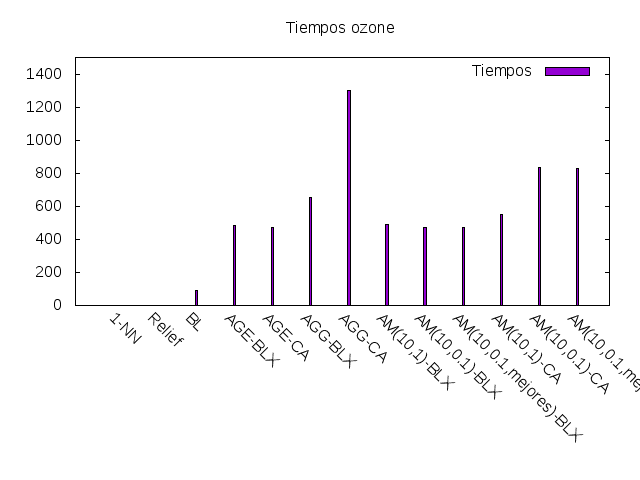
\includegraphics[scale=0.5]{../Graficas/Imagenes/Tiempos/tiempos_ozone.png}
	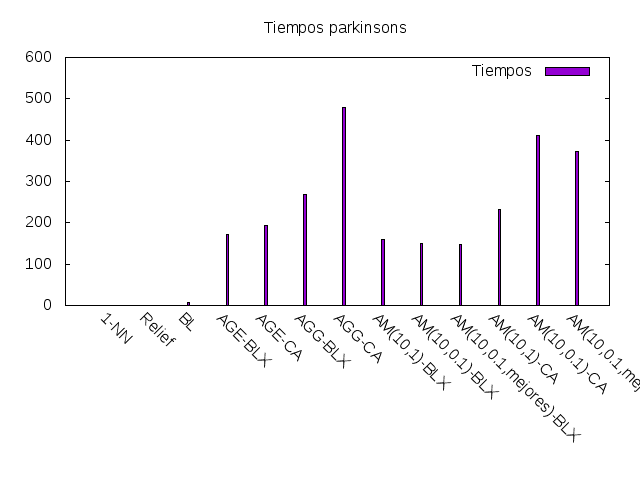
\includegraphics[scale=0.5]{../Graficas/Imagenes/Tiempos/tiempos_parkinsons.png}
	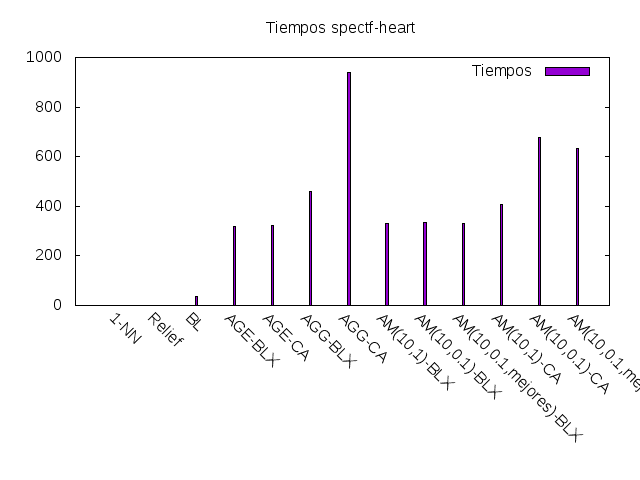
\includegraphics[scale=0.5]{../Graficas/Imagenes/Tiempos/tiempos_spectf-heart.png}
	
	Podemos comprobar que uno de los algoritmos toma mucho más tiempo en todos los ficheros comparado con el resto de los mismos. El algoritmo genético generacional con cruce aritmético llega a consumir más de 1100 segundos en el archivo de datos Ozone, lo cual supone que por ejemplo, el algoritmo genético generacional con cruce aritmético sea una mejor opción en estos conjuntos de datos ya que obtenemos tasas mucho más altas con un coste en tiempo de menos de la mitad con respecto al generacional con cruce aritmético.
	
	\newpage
	
	\subsection{Análisis de la convergencia}
	
	Para comprobar la eficiencia de los algoritmos genéticos he comprobado cómo converge el valor medio de las valoraciones a lo largo de las iteraciones y la generación de las poblaciones. Esto lo he hecho estudiando la media de la valoración (tasa agregada+tasa reducción) de las poblaciones a lo largo del algoritmo obteniendo las siguientes gráficas:
	
	
	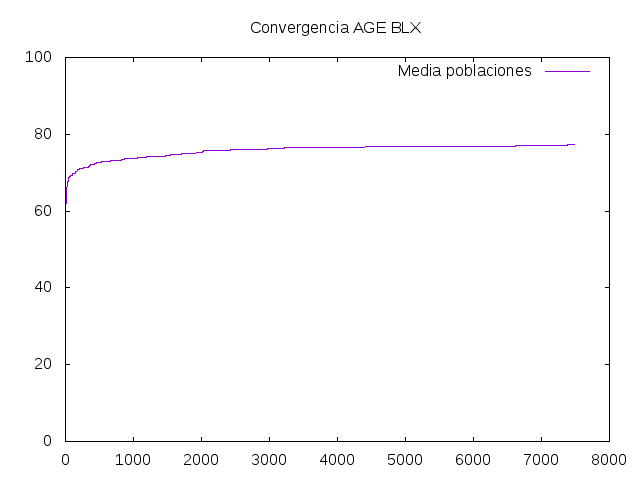
\includegraphics[scale=0.5]{../Graficas/Imagenes/Convergencia/convergencia_estacionario_blx.png}
	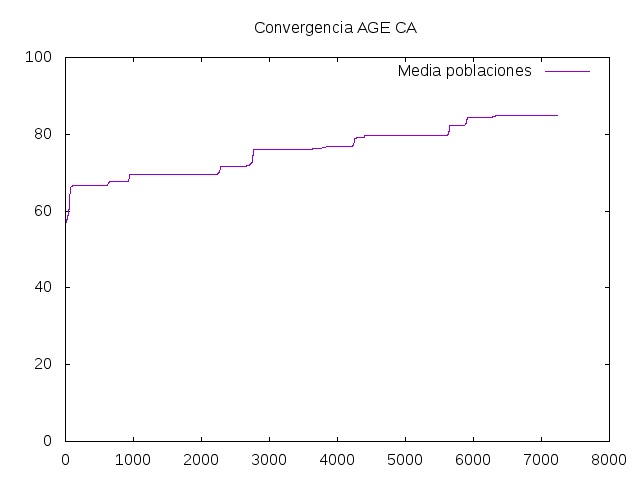
\includegraphics[scale=0.5]{../Graficas/Imagenes/Convergencia/convergencia_estacionario_aritmetico.png}
	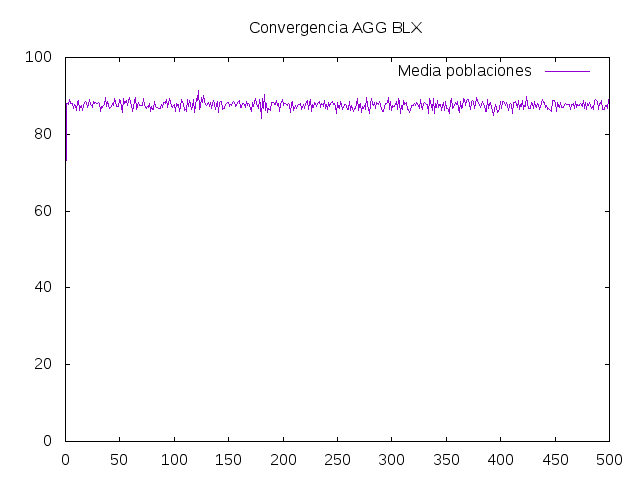
\includegraphics[scale=0.5]{../Graficas/Imagenes/Convergencia/convergencia_generacional_blx.png}
	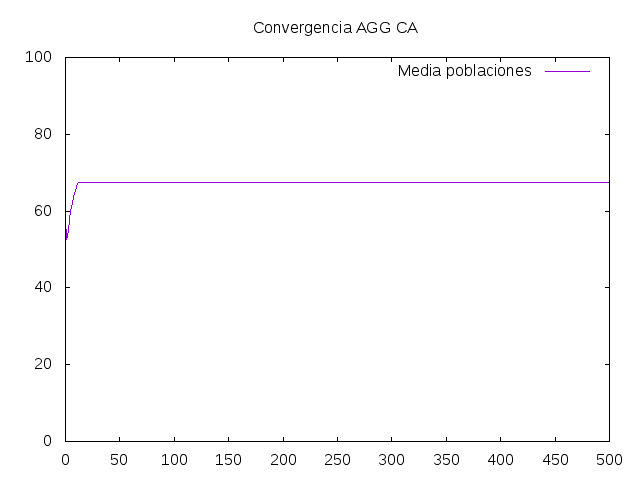
\includegraphics[scale=0.5]{../Graficas/Imagenes/Convergencia/convergencia_generacional_aritmetico.png}

	En estas gráficas observamos que el algoritmo genético estacionario con cruce aritmético ha tenido una convergencia muy progresiva aprovechando todas las iteraciones de las generaciones.
	
	En cambio en los algoritmos genéticos generacionales y el estacionario BLX podemos comprobar que la mayoría de las iteraciones han sido desaprovechadas ya que la población ha convergido muy rápidamente. 
	
	Podemos estudiar la situación que se ha producido en el generacional BLX, ya que la población ha tenido una variación muy pequeña a lo largo del tiempo y además ha ido obteniendo valores en un entorno muy reducido cercano al 90\%.
	
	Por esto podemos decir que una posible mejora para los algoritmos genéticos es que si no obtenemos una mejora tras haber pasado un número dado de generaciones entonces debería parar. Esto nos ahorraría según estas gráficas de convergencia la mayoría de las iteraciones en el genético generacional con cruce aritmético y en el estacionario con cruce BLX. En el caso del generacional BLX sería más complicado saber que debemos parar, ya que los valores ahí si tienen un movimiento notable.
	
	\newpage
	
	\subsection{Calibrando la tasa de mutación}
	
	Durante el transcurso de esta práctica se nos ha pedido que tomemos como ratio de mutación 0.001, es decir, de los nuevos individuos que generamos debemos mutar el 0.001\% de sus genes. Este ratio nos está dejando como resultado una mutación muy pobre de forma que no notamos la diferencia entre dejarla o no hacer mutación alguna.
	
	Por ello, y con el propósito de añadir más diversidad al algoritmo he experimentado cambiando las tasas de mutación de 0.001 a 0.2, obteniendo los siguientes resultados sobre el fichero de datos ozone-320.arff:
	
	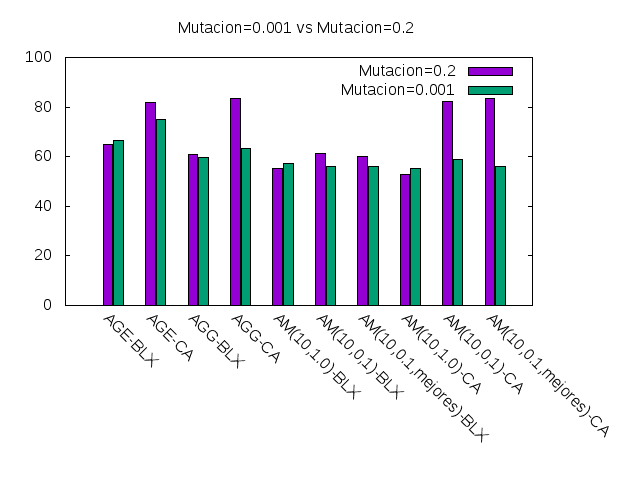
\includegraphics[scale=1]{../Graficas/Imagenes/Mutacion/mutacion.png}

	Podemos observar que en el peor de los casos hemos empeorado un poco los resultados obtenidos con la mutación a 0.001 pero hay 4 algoritmos en los que obtenemos una mejora sustancial al poner la tasa de mutación a 0.2.
	
	Esto es debido a que el ratio de mutación que teníamos previamente no añadía la diversidad suficiente al modelo como para poder escapar de los máximos locales. Ahora al mutar muchos más genes hacemos el cambio suficiente como para pasar por ejemplo en el genético generacional con cruce aritmético de un 63\% de acierto a un 83\%, lo que supone una mejora muy notable.

\end{document}
